\documentclass{beamer}
%\documentclass[handout]{beamer}

% \usepackage{ensislidesOG}
%\usepackage[utf8]{inputenc}
% \usepackage[T1]{fontenc}
\usepackage[english]{babel}
\usepackage[sfdefault]{roboto} 
\usepackage{ulem}
\usepackage{amsfonts}
\usepackage{amsmath}
\usepackage{amssymb}
\usepackage{amsthm}
% \usepackage[frenchstyle]{mathalpha}
% \usepackage[OMLmathsfit]{isomath}
\usepackage{graphicx}
\usepackage{color} % for ps_tex inclusions
\usepackage{fmtcount} % th, e.g. \ordinalnum{4}
\usepackage{booktabs}
\usepackage{tikz}
\usetikzlibrary{fit,positioning,bayesnet}
\usepackage{xr}
\usepackage{hyperref}
\externaldocument[notes-]{notes}
\usetheme{Madrid}
\usecolortheme{seagull}

\newcommand{\itb}{\item[$\bullet$]}
\newcommand{\dps}{\displaystyle}

\def\<{{\guillemotleft}}
\def\>{{\guillemotright}}

\def\vs1{\vspace{1mm}}
\def\v3{\vspace{3mm}}

\newcommand{\II}{\,\mbox{I\hskip -0.600em 1}}

\newcommand{\ME}{{\mathcal E}}
\newcommand{\MN}{{\mathcal N}}

\newcommand{\NN}{\ensuremath{\mathbb{N}}}
\newcommand{\RR}{\ensuremath{\mathbb{R}}}

\newcommand{\card}{\mbox{card}}
\newcommand{\pa}{\mbox{pa}}

\newcommand{\De}{\mbox{De}}
\newcommand{\Nd}{\mbox{Nd}}
\newcommand{\Ne}{\mbox{Ne}}

\newcommand{\indep}{\perp\!\!\!\perp}
\newcommand{\condindep}[3]{#1 \indep #2 \vert #3}
\newcommand{\condindepP}[4]{#1 \indep_{#4} #2 \vert #3}
\newcommand{\ts}[3]{#1_{#2}^{#3}}
\newcommand{\set}[1]{\{#1\}}
\newcommand{\bs}[1]{\boldsymbol{#1}}

\newcommand{\expectation}[2][]{%
\ifthenelse { \equal {#1} {} }%
% Expectation w/o distribution
{\mathbb{E}\left\{#2\right\}}%
% Expectation with distribution
{\mathbb{E}_{#1}\left\{#2\right\}}
}


\title{Learning Probabilities and Causality}

\subtitle{Chapter IV - Probabilistic Principal Component Analysis} % (optional)

\author[Xavi and Thomas]{Xavier Alameda-Pineda and Thomas Hueber}

\institute{Ensimag/Inria/CNRS/Univ. Grenoble-Alpes}


\makeatother
\setbeamertemplate{footline}
{
  \leavevmode%
%   \hbox{%
%   \begin{beamercolorbox}[wd=.4\paperwidth,ht=2.25ex,dp=1ex,center]{author in head/foot}%
%     \usebeamerfont{author in head/foot}\insertshortauthor
%   \end{beamercolorbox}%
%   \begin{beamercolorbox}[wd=.6\paperwidth,ht=2.25ex,dp=1ex,center]{title in head/foot}%
    \usebeamerfont{title in head/foot}\hfill
    \insertframenumber{} / \inserttotalframenumber\hspace*{1ex}
%   \end{beamercolorbox}}%
%   \vskip0pt%
}
\makeatletter
\setbeamertemplate{navigation symbols}{}

\AtBeginSection[]{
  \begin{frame}
  \vfill
  \centering
  \begin{beamercolorbox}[sep=8pt,center,shadow=true,rounded=true]{title}
    \usebeamerfont{title}\insertsectionhead\par%
  \end{beamercolorbox}
  \vfill
  \end{frame}
}

\AtBeginSubsection[]{
  \begin{frame}
  \vfill
  \centering
  \begin{beamercolorbox}[sep=8pt,center,shadow=true,rounded=true]{title}
    \usebeamerfont{title}\insertsectionhead\\---\\\insertsubsectionhead\par%
  \end{beamercolorbox}
  \vfill
  \end{frame}
}

\date{}

\newcommand{\exercise}[2]{\noindent\colorbox{blue!10}{\parbox{0.995\textwidth}{\textbf{Exercise \ref{notes-ex:#1}}: #2}}\\}
\newcommand{\remark}[2]{\noindent\colorbox{red!10}{\parbox{0.995\textwidth}{\textbf{Remark \ref{notes-rmk:#1}}: #2}}\\}


\definecolor{mypurple}{RGB}{200,0,255}

%%%%%%%%%%%%%%%%%%%%%%%%%%%%%%%%%%%%%%%%%%%%%%%%%%%%%%%%%%%%%%

\begin{document}

\begin{frame}
  \titlepage
\end{frame}

\begin{frame}{Contents}
 \tableofcontents
\end{frame}

\section{Motivation}

\begin{frame}{Discrete Latent Variables so far...}

With or without temporal links (GMM on the left and HMM on the right), but always discrete latent variables, $z\in\{1,\ldots,K\}$.
\begin{figure}
%  \centering
 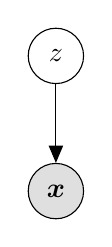
\begin{tikzpicture}[->]
    \node[latent] (z) {$z$};
    \node[obs,below=of z] (x) {$\bs{x}$};
    \edge{z} {x};
\end{tikzpicture}\hspace{2cm}
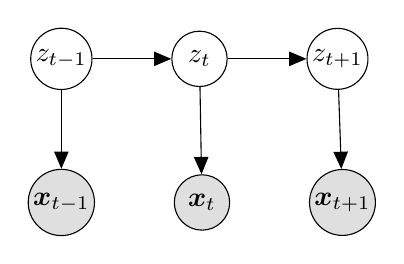
\begin{tikzpicture}[->]
    \node[latent] (zm) {$z_{t-1}$};
    \node[latent,right=of zm] (z) {$z_t$};
    \node[latent,right=of z] (zp) {$z_{t+1}$};
    \node[obs,below=of zm] (xm) {$\bs{x}_{t-1}$};
    \node[obs,right=of xm] (x) {$\bs{x}_t$};
    \node[obs,right=of x] (xp) {$\bs{x}_{t+1}$};
    \edge{zm} {z};
    \edge{z} {zp};
    \edge{zm} {xm};
    \edge{z} {x};
    \edge{zp} {xp};
\end{tikzpicture}
%  \caption{Graphical representation of a GMM (left) and an HMM (right). \label{fig:gmm-hmm}}
\end{figure}

What about continuous latent variables, i.e., $\bs{z}\in\mathbb{R}$ (or multivariate).\vspace{\baselineskip}

The equivalent of the GMM is called PPCA, and the equivalent of the HMM is called linear dynamical system (next chapter).

\end{frame}

\begin{frame}{Model definition}
\remark{ppca-model}{The PPCA model is characterised by:
\begin{itemize}
 \item Two continuous variables: hidden and observed, $\bs{z}\in\mathbb{R}^{d_{\textsc{z}}}$, $\bs{x}\in\mathbb{R}^{d_{\textsc{x}}}$.\\ $d_{\textsc{z}}$ ($d_{\textsc{x}}$) denotes the hidden (observed) dimension, and $d_{\textsc{z}} \ll d_{\textsc{x}}$.
 \item The prior on the latent variable is a standard Gaussian:
 \[
  p(\bs{z}) = \mathcal{N}(\bs{z};\bs{0},\bs{I}).
 \]
 \item The conditional likelihood is a multivariate Gaussian:
 \[
  p(\bs{x}|\bs{z}) = \mathcal{N}(\bs{x};\bs{A}\bs{z}+\bs{b},\nu\bs{I}).
 \]
\end{itemize}}\pause\vspace{3mm}
\exercise{ppca-free-param}{What is the number of free parameters of the PPCA model?}
\end{frame}

\begin{frame}{Intuition about the Generative Process}
Alternatively: $\bs{x}=\bs{A}\bs{z}+\bs{b}+\bs{\epsilon}$ with $\bs{\epsilon}\sim\mathcal{N}(\bs{\epsilon};\bs{0},\nu\bs{I})$, being $\bs{\epsilon} \indep \bs{z}$.\vspace{\baselineskip}

\begin{columns}[b]
 \begin{column}{0.22\textwidth}
 \centering
  
\includegraphics[width=\textwidth]{fig/ppca_generation_1.pdf}\\ $\bs{z}$
 \end{column}\hfill
 \begin{column}{0.22\textwidth}
 \centering
  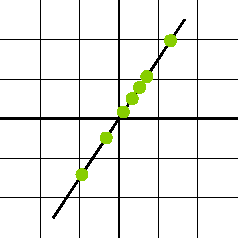
\includegraphics[width=\textwidth]{fig/ppca_generation_2.pdf}\\ $\bs{A}\bs{z}$
 \end{column}\hfill
  \begin{column}{0.22\textwidth}
  \centering
  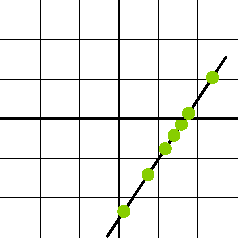
\includegraphics[width=\textwidth]{fig/ppca_generation_3.pdf}\\ $\bs{A}\bs{z}+\bs{b}$
 \end{column}\hfill
  \begin{column}{0.22\textwidth}
  \centering
  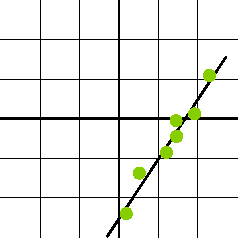
\includegraphics[width=\textwidth]{fig/ppca_generation_4.pdf}\\ $\bs{A}\bs{z}+\bs{b}+\bs{\epsilon}$
 \end{column}
\end{columns}\vspace{\baselineskip}
It's the ``opposite'' direction of standard PCA.
\end{frame}

\begin{frame}{Properties of PCCA}
\exercise{ppca-marginal}{Prove that, given the PPCA model, the marginal of $\bs{x}$ has mean vector $\bs{b}$ and covariance matrix $\bs{A}\bs{A}^\top+\nu\bs{I}$.}\pause\vspace{3mm}

\exercise{ppca-marginal-2}{Prove that the shape of the marginal distribution $p(\bs{x})$ corresponds to the one of a multivariate Gaussian. To do so, first prove that the joint distribution in $\bs{x}$ and $\bs{z}$ can be expressed as:
\[
 p(\bs{x},\bs{z})\stackrel{\bs{x},\bs{z}}{\propto} \exp\left(-\frac{1}{2}\left[ \frac{\|\bs{x}-\bs{b}\|^2}{\nu}-\bs{m}^\top\bs{\Omega}^{-1}\bs{m}\right]\right)\mathcal{N}(\bs{z};\bs{m},\bs{\Omega}),
\]
with
\[
 \bs{\Omega} = \left(\frac{\bs{A}^\top\bs{A}}{\nu}+\bs{I}\right)^{-1} \qquad \bs{m}=\bs{\Omega}\left(\frac{\bs{A}^\top(\bs{x}-\bs{b})}{\nu}\right) .
\]
}\pause\vspace{3mm}
Are these two results compatible?
\end{frame}

\begin{frame}{Woodbury Matrix Inversion Lemma}
The answer is yes! It is trivial for the mean, but for the covariance we need the following result:\vspace{3mm}
\remark{woodbury}{For matrices $\bs{D}\in\mathbb{R}^{n\times n}$, $\bs{U}\in\mathbb{R}^{n\times m}$, $\bs{C}\in\mathbb{R}^{m\times m}$ and $\bs{V}\in\mathbb{R}^{m\times n}$, the following identity holds:
\[
 (\bs{D} + \bs{U}\bs{C}\bs{V})^{-1} = \bs{D}^{-1}-\bs{D}^{-1}\bs{U}(\bs{C}^{-1}+\bs{V}\bs{D}^{-1}\bs{U})^{-1}\bs{V}\bs{D}^{-1}.
\]
}\vspace{3mm}

\exercise{woodbury}{Prove the Woodbury matrix inversion lemma.}

\end{frame}

\section{The EM for PPCA}

\begin{frame}{The $\mathcal{Q}$ function}
As usual, we assume a set of observations $\bs{X}=\{\bs{x}_1,\ldots,\bs{x}_N\}$ and associated latents $\bs{Z}=\{\bs{z}_1,\ldots,\bs{z}_N\}$. The parameters of the model are $\bs{\Theta}=\{\bs{A},\bs{b},\nu\}$. \vspace{3mm}

Given their initialisation, $\bar{\bs{\Theta}}=\{\bar{\bs{A}},\bar{\bs{b}},\bar{\nu}\}$, the EM algorithm considers the expecteded complete-data log-likelihood:
\[
 \mathcal{Q}(\bs{\Theta},\bar{\bs{\Theta}}) =\mathbb{E}_{p(\bs{Z}|\bs{X};\bar{\bs{\Theta}})} \log p(\bs{X},\bs{Z};\bs{\Theta})  = \sum_{n=1}^N \mathbb{E}_{p(\bs{z}_n|\bs{x}_n;\bar{\bs{\Theta}})} \log p(\bs{x}_n,\bs{z}_n;\bs{\Theta}).
\]\vspace{3mm}

What are $p(\bs{z}_n|\bs{x}_n;\bar{\bs{\Theta}})$ and $\mathbb{E}_{p(\bs{z}_n|\bs{x}_n;\bar{\bs{\Theta}})} \log p(\bs{x}_n,\bs{z}_n;\bs{\Theta})$?
\end{frame}


\begin{frame}{Towards the E step}
We recall that $p(\bs{z}_n|\bs{x}_n;\bar{\bs{\Theta}})=\mathcal{N}(\bs{z}_n;\bar{\bs{m}}_n,\bar{\bs{\Omega}})$ with:
\[
\bar{\bs{\Omega}} = \left(\frac{\bar{\bs{A}}^\top\bar{\bs{A}}}{\bar{\nu}}+\bs{I}\right)^{-1} \quad\text{and}\quad \bar{\bs{m}}_n=\bar{\bs{\Omega}}\left(\frac{\bar{\bs{A}}^\top(\bs{x}_n-\bar{\bs{b}})}{\bar{\nu}}\right) .
\]\vspace{3mm}

In order to compute $\mathcal{Q}$ we will need:\vspace{3mm}
\exercise{expectation-log-gaussian}{The following two formulae hold:
\[
 \expectation[\mathcal{N}(\bs{z};\bs{\mu},\bs{\Sigma})]{\bs{A}\bs{z}} = \bs{A}\bs{\mu} \quad\text{and}\quad \expectation[\mathcal{N}(\bs{z};\bs{\mu},\bs{\Sigma})]{\bs{z}^\top\bs{\Lambda}\bs{z}} = \bs{\mu}^\top\bs{\Lambda}\bs{\mu} + \textrm{Tr}(\bs{\Lambda}\bs{\Sigma}).  
\]
}\vspace{2mm}
\end{frame}

\begin{frame}{The E step for PPCA}
 \exercise{ppca-q-term}{Show that the $n$-th term of the sum of the $\mathcal{Q}$ function for PPCA writes:
\begin{align*}
 &\expectation[\mathcal{N}(\bs{z}_n;\bar{\bs{m}}_n,\bar{\Omega})]{\log \mathcal{N}(\bs{x}_n;\bs{A}\bs{z}_n+\bs{b},\nu\bs{I})\mathcal{N}(\bs{z}_n;\bs{0},\bs{I})}\\
 &\qquad\stackrel{\bs{\Theta}}{=} -\frac{1}{2}\left(d_{\textsc{x}}\log\nu + \frac{1}{\nu}\|\bs{x}_n-\bs{A}\bar{\bs{m}}_n-\bs{b}\|^2 + \frac{1}{\nu}\textrm{Tr}(\bs{A}^\top\bs{A}\bar{\bs{\Omega}})\right),
\end{align*}
where the notation $ \stackrel{\bs{\Theta}}{=} $ means equality up to an additive constant that does not depend on $\bs{\Theta}$.
}\pause\vspace{2mm}

Therefore the $\mathcal{Q}$ writes:
\begin{align*}
 \mathcal{Q}(\bs{\Theta},\bar{\bs{\Theta}}) \stackrel{\bs{\Theta}}{=} -\frac{N}{2}\left(d_{\textsc{x}}\log\nu  + \frac{1}{\nu}\textrm{Tr}(\bs{A}^\top\bs{A}\bar{\bs{\Omega}}) + \frac{1}{N\nu}\sum_{n=1}^N\|\bs{x}_n-\bs{A}\bar{\bs{m}}_n-\bs{b}\|^2\right)
\end{align*}
\end{frame}

\begin{frame}{The M step for PPCA}

{\small \begin{align*}
 \mathcal{Q}(\bs{\Theta},\bar{\bs{\Theta}}) \stackrel{\bs{\Theta}}{=} -\frac{N}{2}\left(d_{\textsc{x}}\log\nu  + \frac{1}{\nu}\textrm{Tr}(\bs{A}^\top\bs{A}\bar{\bs{\Omega}}) + \frac{1}{N\nu}\sum_{n=1}^N\|\bs{x}_n-\bs{A}\bar{\bs{m}}_n-\bs{b}\|^2\right)
\end{align*}}
  \exercise{optimal-nu-ppca}{
 The optimal value for $\nu$ writes:
 \[
  \nu^* = \frac{1}{d_{\textsc{x}}}\left(\textrm{Tr}(\bs{A}^\top\bs{A}\bar{\bs{\Omega}}) + \frac{1}{N} \sum_{n=1}^N\|\bs{x}_n-\bs{A}\bar{\bs{m}}_n-\bs{b}\|^2\right).
 \]\pause
 Regarding the other two parameters, nulling out their respective derivatives yields:
 \begin{align*}
  \bs{A} = (\bs{S}_{\textsc{xm}}-\bs{b}\bs{S}_{\textsc{m}}^\top)\bs{S}^{-1}_2 \quad\text{and}\quad \bs{b} = \bs{S}_{\textsc{x}}-\bs{A}\bs{S}_{\textsc{m}},
 \end{align*}
where $\bs{S}_{\textsc{x}}=\frac{1}{N}\sum_{n=1}^N\bs{x}_n\in\mathbb{R}^{d_{\textsc{x}}}$, $\bs{S}_{\textsc{m}}=\frac{1}{N}\sum_{n=1}^N \bar{\bs{m}}_n\in\mathbb{R}^{d_{\textsc{z}}}$, $\bs{S}_{\textsc{xm}} = \frac{1}{N}\sum_{n=1}^N \bs{x}_n\bar{\bs{m}}_n^\top\in\mathbb{R}^{d_{\textsc{x}}\times d_{\textsc{z}}}$, $\bs{S}_2=\frac{1}{N}\sum_{n=1}^N \bar{\bs{m}}_n\bar{\bs{m}}_n^\top + \bar{\Omega}\in\mathbb{R}^{d_{\textsc{z}}\times d_{\textsc{z}}}$. 
}
\end{frame}

\begin{frame}{The M step for PPCA (c'ed)}
 This means that the optimal values of $\bs{A}$ and $\bs{b}$ must be found by solving a linear system of equations, yielding:
\[
 \bs{A}^* = (\bs{S}_{\textsc{xm}}-\bs{S}_{\textsc{x}}\bs{S}_{\textsc{m}})\bs{S}_2^{-1}(\bs{I}-\bs{S}_m\bs{S}_m^\top\bs{S}_2^{-1})^{-1}, \quad\text{and}\quad \bs{b}^* = \bs{S}_{\textsc{x}}-\bs{A}^*\bs{S}_{\textsc{m}}.
\]\vspace{3mm}

The final EM algorithm starts with $\bar{\bs{\Theta}}$ and alternates between:
\begin{itemize}
 \item Computing $\bar{\bs{m}}_n,\bar{\bs{\Omega}}, \forall n$.
 \item Computing $\nu^*$, $\bs{A}^*$ and $\bs{b}^*$, and setting $\bar{\bs{\Theta}}$ to these values.
\end{itemize}
Return $\bar{\bs{\Theta}}$ after some convergence criterion is met.\vspace{6mm}

Which are the parameters of the model?

\end{frame}

\section{The linear-Gaussian model}

\begin{frame}{Generalising PPCA}
\remark{linear-gaussian}{The so-called \textbf{linear Gaussian} model, which is actually afine, is defined as:
 \[
  p(\bs{z}) = \mathcal{N}(\bs{z};\bs{\mu},\bs{\Sigma}) \qquad 
  p(\bs{x}|\bs{z}) = \mathcal{N}(\bs{x};\bs{A}\bs{z}+\bs{b},\bs{L}),
 \]
 $\bs{\mu}\in\mathbb{R}^{d_{\textsc{z}}}$, $\bs{\Sigma}\in\mathbb{R}^{d_{\textsc{z}}\times d_{\textsc{z}}}$, $\bs{A}\in\mathbb{R}^{d_{\textsc{x}}\times d_{\textsc{z}}}$, $\bs{b}\in\mathbb{R}^{d_{\textsc{x}}}$ and $\bs{L}\in\mathbb{R}^{d_{\textsc{x}}\times d_{\textsc{x}}}$. 
}\vspace{5mm}

More general, since the PPCA model is a particular case with $\bs{L}=\nu\bs{I}$, $\bs{\mu}=\bs{0}$, and $\bs{\Sigma}=\bs{I}$.\vspace{5mm}

\exercise{linear-gaussian-free-param}{What are the number of free parameters of this model?}\vspace{2mm}\pause It's $d_{\textsc{z}}$ for $\bs{\mu}$, $d_{\textsc{x}}$ for $\bs{b}$, $d_{\textsc{z}}\times d_{\textsc{x}}$ for $\bs{A}$. For the covariance matrices we have $d_{\textsc{z}}(d_{\textsc{z}}+1)/2$ for $\bs{\Sigma}$ and $d_{\textsc{x}}(d_{\textsc{x}}+1)/2$ for $\bs{L}$, since they are symmetric.\vspace{2mm}\\
\textbf{Altogether} they sum up to $d_{\textsc{x}}+d_{\textsc{z}}$ plus $(d_{\textsc{x}}+d_{\textsc{z}})(d_{\textsc{x}}+d_{\textsc{z}}+1)/2$.
\end{frame}

\begin{frame}{Properties of the linear-Gaussian model}
\exercise{linear-gaussian}{Using the Gaussian completion, prove the following results. For the posterior distribution $p(\bs{z}|\bs{x}) = \mathcal{N}(\bs{z};\bs{m},\bs{\Omega})$:
\[
 \bs{\Omega}^{-1} = \bs{\Sigma}^{-1}+\bs{A}^\top\bs{L}^{-1}\bs{A} \quad\text{and}\quad \bs{m}=\bs{\Omega}(\bs{\Sigma}^{-1}\bs{\mu}+\bs{A}^\top\bs{L}^{-1}(\bs{x}-\bs{b})). 
\]
For the marginal distribution:
\[
 p(\bs{x}) = \mathcal{N}(\bs{x};\bs{A}\bs{\mu}+\bs{b},\bs{A}\bs{\Sigma}\bs{A}^\top + \bs{L}).
\]
For the joint distribution $p(\bs{x},\bs{z})$:
\[
 \mathcal{N} \left(\left(\begin{array}{c}\bs{x}\\\bs{z}\end{array}\right); \left(\begin{array}{c}\bs{L}^{-1}\bs{b}\\\bs{\Sigma}^{-1}\bs{\mu}+\bs{A}^\top\bs{L}^{-1}\bs{b}\end{array}\right),\left(\begin{array}{cc}\bs{L}^{-1} & \bs{L}^{-1}\bs{A}\\\bs{A}^\top\bs{L}^{-1} & \bs{\Sigma}^{-1}+\bs{A}^\top\bs{L}^{-1}\bs{A}\end{array}\right)\right)
\]
}
\end{frame}




\end{document}

